%template1.tex
%The following LaTeX source file represents the simplest kind of slide presentation; no overlays, no included graphics. Substitute your favorite style for ``pascal''. To create the PDF file template1.pdf, (1) be sure to use the prosper class, then (2) execute the command latex template1.tex, and (3) the command dvipdf template1.dvi.

%%%%%%%%%%%%%%%%%%%%%%%%%%%%%%% template1.tex %%%%%%%%%%%%%%%%%%%%%%%%%%%%%%%%%%%
\documentclass[a4paper,blends,pdf,colorBG,slideColor]{prosper}
% definitions for slides for CSC544
% Lutz Hamel, (c) 2007

\hypersetup{pdfpagemode=FullScreen}

\usepackage{times}
\usepackage{latexsym}
\usepackage{alltt}
\usepackage{booktabs}
\usepackage{amsmath}
\usepackage{amsopn}
\usepackage{amsfonts}
\usepackage{amssymb}
%\usepackage[usenames]{color}

\def\sign{\qopname\relax{no}{sign}}
\def\argmax{\qopname\relax{no}{argmax}}
\def\argmin{\qopname\relax{no}{argmin}}

\newcommand{\grad}{\ensuremath{\nabla}} 
\newcommand{\loss}{\ensuremath{{\cal L}}}
\newcommand{\err}{\mbox{err}}
\newcommand{\mse}{\mbox{mse}}
\newcommand{\acc}{\mbox{acc}}
\newcommand{\Integer}{\ensuremath{\mathbb{N}}}
\newcommand{\size}[1]{{|{#1}|}}
\newcommand{\Rnspace}[1]{\ensuremath{\mathbb{R}^{#1}}}
\newcommand{\Real}{\ensuremath{\mathbb{R}}}
\newcommand{\mytt}[1]{{\small\tt{#1}}}
\newcommand{\textemph}[1]{{\em #1}}
\newcommand{\suchthat}{\mid}
\newcommand{\orbar}{\;|\;}
\newcommand{\bs}[1]{\begin{slide}{#1}\ptsize{8}}
\newcommand{\es}{\end{slide}}
\newcommand{\co}{\,\colon\;}
\newcommand{\pair}[2]{\ensuremath{( {#1}, {#2} )}}
\newcommand{\model}[1]{\hat{#1}}
\newcommand{\ul}[1]{{\bf\em #1}}
\newcommand{\ol}{\overline}
\newcommand{\definition}[1]{{\bf Definition: }{\em #1}}
\newcommand{\example}[1]{{\bf Example: }{#1}}
\newcommand{\abs}[1]{|{#1}|}
\newcommand{\mytab}{\makebox[.1in]{}}

\newcommand{\fdef}[1]{
\begin{center}
\fbox{
\begin{minipage}{3.5in}
{\bf Definition:}
{#1}
\end{minipage}
}
\end{center}
}

\newcommand{\fframe}[1]{
\begin{center}
\fbox{
\begin{minipage}{3.5in}
{#1}
\end{minipage}
}
\end{center}
}

\newcommand{\nframe}[1]{
\begin{center}
\begin{minipage}{3.5in}
{#1}
\end{minipage}
\end{center}
}

\newenvironment{Rcode}
	{
		\scriptsize
		\begin{quote}
		\begin{alltt}
	}
	{
		\end{alltt}
		\end{quote}
	}




\begin{document}

\bs{Regression as Machine Learning}
Given
\begin{itemize}
\item A data universe $X$.
\item A sample set $S$ where $S \subset X$.
\item Some target function $f\co X \rightarrow {\color{red}\Real}$.
\item A training set $D$, where
$
D = \{ (x ,y) \suchthat x \in S \text{ and } y = f(x)\}.
$
\end{itemize}
Compute a model $\model{f}\co X \rightarrow {\color{red}\Real}$ using $D$ such that,
\begin{equation*}
\model{f}(x) \cong f(x),
\end{equation*}
for all $x \in X$.

\vspace{.1in}

{\bf Observation:}  Same as machine learning in classification except for the co-domains 
of the target function and the model.

{\bf Question:} How do we compute the model?

\es

\bs{Statistical Approaches}
\small
Assume we have a regression training set of the form,
\begin{equation*}
D = \{(\ol{x}_1,y_1), (\ol{x}_2,y_2),\ldots,(\ol{x}_l,y_l)\} \subset \Rnspace{n} \times {\color{red}\Real}.
\end{equation*}
Then let  $\model{f}(\ol{x})$
be a regression model on $D$,
where the quantity
\begin{equation*}
\rho_i = y_i - \model{f}(\ol{x}_i)
\end{equation*}
for $(\ol{x}_i,y_i)\in D$ is called a {\em residual} and measures the difference between
model output and the actual observation.  Observe that the residual depends on the model 
we choose.

In linear regression we compute the minimum \textemph{sum of squared errors}
in order to obtain an optimal model,
\begin{equation*}
\min \sum_{i = 1}^l \rho_i^2 = \min_{\model{f}} \sum_{i=1}^l \left( y_i - \model{f}(\ol{x}_i)\right )^2,
\end{equation*}
with $(\ol{x}_i,y_i)\in D$.

Rewriting the above optimization problem slightly we obtain,
\begin{equation*}
\model{f}^* = \argmin_{\model{f}} \sum_{i=1}^l \left( y_i - \model{f}(\ol{x}_i)\right )^2.
\end{equation*}
\es

\bs{Statistical Approaches}
\vspace{.2in}
\begin{center}
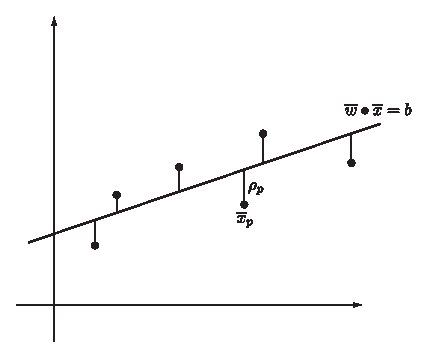
\includegraphics[height=50mm]{figures/fig12-01.eps}
\end{center}

Linear regression with residuals, here the point $\ol{x}_p$ is an observation and $\rho_p$
is the residual at that observation given the model $\ol{w}\bullet\ol{x}=b$.
\es


\bs{Example}
\begin{center}
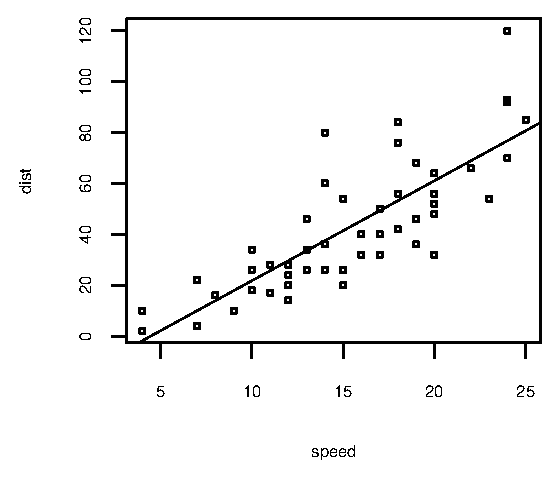
\includegraphics[height=50mm]{figures/fig12-02.eps}
\end{center}

\begin{Rcode}
> data(cars)
> model <- {\color{red}lm}(cars$dist ~ ., data = cars)
> plot(cars)
> abline(model)
\end{Rcode}

\es


\bs{Maximum Margin Machines}
\begin{center}
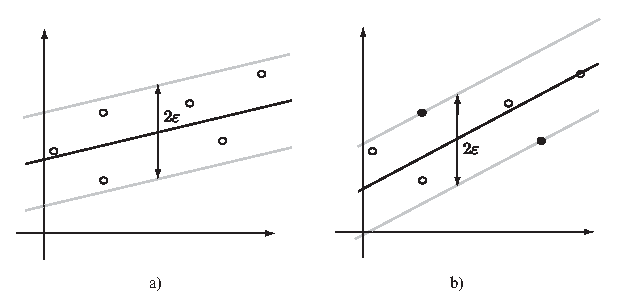
\includegraphics[height=45mm]{figures/fig12-03.eps}
\end{center}

Solving regression problems with linear models using a $\varepsilon$ hyper-tube.
In part a) we show a regression model where all observations are within the hyper-tube depicted with 
the light gray lines,
part b) depicts the optimal regression model with a maximum margin.
\es

\bs{Maximum Margin Machines}

\fframe{{\bf Proposition:} Given the regression training set,
\begin{equation*}
D = \{(\ol{x}_1,y_1),(\ol{x}_2,y_2),\ldots,(\ol{x}_l,y_l)\} \subseteq \Rnspace{n} \times \Real,
\end{equation*}
where the optimal maximum margin regression model can be computed as the optimization, 
\begin{equation*}
\min \phi(\ol{w},b) = \min_{\ol{w},b}\frac{1}{2}\ol{w}\bullet\ol{w}
\end{equation*}
such that the constraints,
\begin{align*}
y_i - \model{f}(\ol{x}_i) &\le \varepsilon,\\
\model{f}(\ol{x}_i) - y_i &\le \varepsilon,
\end{align*}
are satisfied for $i = 1,\ldots,l$ and where $\model{f}(\ol{x}) = \ol{w}\bullet\ol{x} - b$.
}

The constraints specify the the solution must be a model such that the observations are contained
within the $\varepsilon$-tube, $\abs{y_i - \model{f}(\ol{x}_i)} \le \varepsilon$.
\es


\bs{Maximum Margin Machines}
\small
In real-world settings it is unrealistic to assume that all observations will fall into a reasonable
$\varepsilon$-tube, (e.g. cars data set). 

For observations that fall outside the hyper-tube with a fixed value of $\varepsilon$ we introduce correction terms or \textemph{slack variables} that tell us how much of a correction is needed in order for these observations to be moved
into the hyper-tube.


\begin{center}
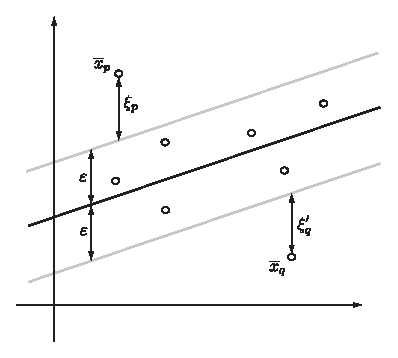
\includegraphics[height=40mm]{figures/fig12-04.eps}
\end{center}
Linear maximum margin regression with slack variables.
\es

\bs{Maximum Margin Machines}

We define the slack variables formally as,
\begin{align*}
\xi_i &= \left \{
	\begin{array}{ll}
	0 & \text{if $y_i - \model{f}(\ol{x}_i) \le \varepsilon$},\\
	\abs{y_i - \model{f}(\ol{x}_i)} - \varepsilon & \text{otherwise},
	\end{array}
	\right .\\
\xi_i' &= \left \{
	\begin{array}{ll}
	0 & \text{if $\model{f}(\ol{x}_i) - y_i \le \varepsilon$},\\
	\abs{y_i - \model{f}(\ol{x}_i)} - \varepsilon & \text{otherwise},
	\end{array}
	\right .	
\end{align*}
for $i = 1,\ldots,l$ with $(\ol{x}_i,y_i)\in D$.

Here the slack variables $\xi_i$ are zero except for observations that lie above the hyper-tube.
Conversely, the slack variables $\xi_i'$ are zero except for observations that lie below the
hyper-tube.

\es

\bs{Maximum Margin Machines}
\small
We can now state regression with maximum margin machines as follows,

\fframe{{\bf Proposition:} Given a regression training set,
\begin{equation*}
D = \{(\ol{x}_1,y_1),(\ol{x}_2,y_2),\ldots,(\ol{x}_l,y_l)\} \subseteq \Rnspace{n} \times \Real,
\end{equation*}
we can compute the optimal regression model $\model{f}^*(\ol{x}) = \ol{w}^*\bullet\ol{x} - b^*$
as the optimization
\begin{align*}
\min \phi(\ol{w},b,\ol{\xi},\ol{\xi}') &=
	\min_{\ol{w},b,\ol{\xi},\ol{\xi}'} \frac{1}{2}\ol{w}\bullet\ol{w} +
	C \sum_{i = 1}^l( \xi_i + \xi_i'), \\
\intertext{such that the constraints,}
y_i - \model{f}(\ol{x}_i) & \le \xi_i + \varepsilon ,\\
\model{f}(\ol{x}_i) -y_i &\le \xi_i' + \varepsilon,\\
0 &\le \xi_i, \xi_i' ,
\end{align*}
for $i = 1,\ldots,l$ hold with $\model{f}(\ol{x}) = \ol{w}\bullet\ol{x} - b$.
}

In the above proposition the penalty constant $C$ modulates the trade-off between margin maximization and
the minimization of the slack variables.
\es

\bs{Regression with SVMs}
Recall that SVMs are the dual to maximum margin machines.  
Also recall that we can derive the dual to maximum margin
optimization by constructing the Lagrangian optimization,
\begin{align*}
\max_{\ol{\alpha}} \min_{\ol{x}} L(\ol{\alpha},\ol{x}) &= \max_{\ol{\alpha}} \min_{\ol{x}} \left (\phi(\ol{x}) - \sum_{i=1}^l \alpha_i g_i(\ol{x})\right),\\
\intertext{subject to the constraints,}
\alpha_i &\ge 0,
\end{align*}
for $i = 1,\ldots,l$.
Here $g_i(\ol{x}) \geq 0$ are inequality constraints and the variables $\ol{\alpha}$ and $\ol{x}$
are called the dual and primal variables of the optimization problem, respectively.

\es

\bs{Regression with SVMs}

As a first step in constructing the Lagrangian optimization we derive our inequality constraints.
This is easily done by slightly rewriting the constraints appearing in the primal optimization problem,
\begin{align*}
\xi_i + \varepsilon- y_i + \model{f}(\ol{x}_i)  &\geq 0,\\
\xi_i' + \varepsilon - \model{f}(\ol{x}_i)  + y_i  &\geq 0, \\
\xi_i &\geq 0, \\
\xi_i' &\geq 0.
\end{align*}
The four sets of inequality constraints imply that we have to introduce {\em four sets of dual variables} into our
Lagrangian optimization.
\es

\bs{Regression with SVMs}
\small
Our Lagrangian:
\begin{multline*}
\max_{\ol{\alpha},\ol{\alpha}',\ol{\beta},\ol{\beta}'}
\min_{\ol{w},b,\ol{\xi},\ol{\xi}'} 
L(\ol{\alpha},\ol{\alpha}',\ol{\beta},\ol{\beta}',\ol{w},b,\ol{\xi},\ol{\xi}') =\\
\begin{aligned}
\max_{\ol{\alpha},\ol{\alpha}',\ol{\beta},\ol{\beta}'}
\min_{\ol{w},b,\ol{\xi},\ol{\xi}'} 
	&\left ( \frac{1}{2}\ol{w}\bullet\ol{w} +
	C \sum_{i = 1}^l ( \xi_i + \xi_i') \right . \\
&\quad -	\sum_{i = 1}^l \alpha_i \left(\xi_i + \varepsilon- y_i + \model{f}(\ol{x}_i)\right)  \\
&\quad -	\sum_{i = 1}^l \alpha_i'\left(\xi_i' + \varepsilon - \model{f}(\ol{x}_i)  + y_i \right)  \\
&\quad -	\sum_{i = 1}^l \beta_i \xi_i \\
&\quad -	\left . \sum_{i = 1}^l \beta_i' \xi_i' \right ),
\end{aligned}
\end{multline*}
subject to the constraints,
\begin{equation*}
\alpha_i,\alpha_i',\beta_i,\beta_i' \ge 0,
\end{equation*}
for $i = 1,\ldots,l$ and where $\model{f}(\ol{x}) =  \ol{w}\bullet\ol{x} - b$.
\es

\bs{Regression with SVMs}
\vspace{.2in}
Given a solution to the Lagrangian optimization,
\begin{equation*}
\max_{\ol{\alpha},\ol{\alpha}',\ol{\beta},\ol{\beta}'}
\min_{\ol{w},b,\ol{\xi},\ol{\xi}'} L(\ol{\alpha},\ol{\alpha}',\ol{\beta},\ol{\beta}',\ol{w},b,\ol{\xi},\ol{\xi}') =
L(\ol{\alpha}^*,\ol{\alpha}'^*,\ol{\beta}^*,\ol{\beta}'^*,\ol{w}^*,b^*,\ol{\xi}^*,\ol{\xi}'^*),
\end{equation*}
we know that  the KKT conditions need to hold.
\es

\bs{KKT Conditions}
\tiny\begin{align*}
\frac{\partial L(\ol{\alpha}^*,\ol{\alpha}'^*,\ol{\beta}^*,\ol{\beta}'^*,\ol{w}^*,b^*,\ol{\xi}^*,\ol{\xi}'^*)}{\partial \ol{w}}  &=  \ol{0},\\
\frac{\partial L(\ol{\alpha}^*,\ol{\alpha}'^*,\ol{\beta}^*,\ol{\beta}'^*,\ol{w}^*,b^*,\ol{\xi}^*,\ol{\xi}'^*)}{\partial b}  &=  0,\\
\frac{\partial L(\ol{\alpha}^*,\ol{\alpha}'^*,\ol{\beta}^*,\ol{\beta}'^*,\ol{w}^*,b^*,\ol{\xi}^*,\ol{\xi}'^*)}{\partial \xi_i}  &=  0,\\
\frac{\partial L(\ol{\alpha}^*,\ol{\alpha}'^*,\ol{\beta}^*,\ol{\beta}'^*,\ol{w}^*,b^*,\ol{\xi}^*,\ol{\xi}'^*)}{\partial \xi_i'}  &=  0,\\
\alpha_i^* \left(\xi_i^* + \varepsilon- y_i + \model{f}^*(\ol{x}_i)\right) &= 0,\\
\alpha_i'^* \left(\xi_i'^* + \varepsilon - \model{f}^*(\ol{x}_i)  + y_i \right) &= 0, \\
\beta_i^*\xi_i^* &= 0, \\
\beta_i'^*\xi_i'^* &= 0,\\
\xi_i^* + \varepsilon- y_i + \model{f}^*(\ol{x}_i) &\geq 0,\\
\xi_i'^* + \varepsilon - \model{f}^*(\ol{x}_i)  + y_i  &\geq 0, \\
\xi_i^*,\xi_i'^* &\geq 0, \\
\alpha_i,\alpha_i'&\geq 0,\\
\beta_i^*,\beta_i'^* &\geq 0,
\end{align*}
where $i = 1,\ldots,l$ and $\model{f}^*(\ol{x}) = \ol{w}^*\bullet\ol{x} - b^*$ is
the optimal regression function.

\es

\bs{Regression with SVMs}

\scriptsize

\fframe{{\bf Proposition:} Given a regression training set,
\begin{equation*}
D = \{(\ol{x}_1,y_1),(\ol{x}_2,y_2),\ldots,(\ol{x}_l,y_l)\} \subseteq \Rnspace{n} \times \Real,
\end{equation*}
then we can compute the optimal support vector regression model $\model{f}^*(\ol{x}) = \ol{w}^*\bullet\ol{x} - b^*$
with
\begin{equation*}
\begin{aligned}
\max_{\ol{\alpha},\ol{\alpha}'} \phi'(\ol{\alpha},\ol{\alpha}') =
	 \max_{\ol{\alpha},\ol{\alpha}'} & \left (\frac{1}{2} \sum_{i = 1}^l \sum_{j = 1}^l(\alpha_i - \alpha_i')(\alpha_j - \alpha_j')\ol{x}_i\bullet\ol{x}_j \right . \\
&\left .\quad	+ \sum_{i = 1}^l y_i(\alpha_i - \alpha_i')
	- \varepsilon \sum_{i = 1}^l (\alpha_i + \alpha_i')\right ),
\end{aligned}
\end{equation*}
subject to the constraints,
$
\sum_{i = 1}^l (\alpha_i - \alpha_i') = 0 \text{ and }C \geq \alpha_i, \alpha_i' \geq 0,
$
for $i = 1,\dots,l$ where
\begin{align*}
\ol{w}^* &= \sum_{i = 1}^l (\alpha_i^* - \alpha_i'^*)\ol{x}_i,\\
b^* &= \frac{1}{l}\sum_{i = 1}^l\ol{w}^* \bullet \ol{x}_i - y_i.
\end{align*}
}
\es


\bs{Regression with SVMs}
As in the case of classification it is perhaps interesting to look at a solution to the optimization
in terms of the complementarity conditions,
\begin{align*}
\alpha_i^* \left(\xi_i^* + \varepsilon- y_i + \model{f}^*(\ol{x}_i)\right) &= 0,\\
\alpha_i'^* \left(\xi_i'^* + \varepsilon - \model{f}^*(\ol{x}_i)  + y_i \right) &= 0,\\
\beta_i^*\xi_i^* &= 0, \\
\beta_i'^*\xi_i'^* &= 0,
\end{align*}
and the fact that a support vector is now described by the coefficient $(\alpha_i - \alpha_i') \ne 0$.


\es

\bs{Regression with SVMs}

First we show that if some point $\ol{x}_i$ is strictly contained in the $\varepsilon$-tube then it is not a support vector.
If the point is strictly within the $\varepsilon$-tube then the following is true
\begin{align*}
\varepsilon &> y_i -  \model{f}(\ol{x}_i) ,\\
\varepsilon &>  \model{f}(\ol{x}_i)  - y_i . \\
\end{align*}
and $\xi_i,\xi_i' = 0$.
This means that the following holds,
\begin{align*}
\xi_i + \varepsilon- y_i + \model{f}(\ol{x}_i)  &> 0,\\
\xi_i' + \varepsilon - \model{f}(\ol{x}_i)  + y_i  &> 0. \\
\end{align*}
This implies that $\alpha_i=0$ and $\alpha'_i=0$ in order for the complimentarity conditions to be satisfied.

It  follows that the coefficient $ (\alpha_i - \alpha_i') = 0$, thus a point $\ol{x}_i$ contained
in the $\varepsilon$-tube is {\em not} a support vector.
\es

\bs{Regression with SVMs}
Now consider a point $\ol{x}_i$ that sits right on the $\varepsilon$-tube boundary, then either
\begin{align*}
\xi_i + \varepsilon- y_i + \model{f}(\ol{x}_i)  &= 0,\\
\xi_i' + \varepsilon - \model{f}(\ol{x}_i)  + y_i  &> 0, \\
\end{align*}
or
\begin{align*}
\xi_i + \varepsilon- y_i + \model{f}(\ol{x}_i)  &> 0,\\
\xi_i' + \varepsilon - \model{f}(\ol{x}_i)  + y_i  &= 0, \\
\end{align*}
with $\xi_i,\xi'_i=0$.

(the point $\ol{x}_i$ cannot be on both boundaries at the same time)

This in turn implies that either $0 < \alpha_i< C$ and $\alpha'_i = 0$ or 
$0 < \alpha'_i< C$ and $\alpha_i = 0$.

Note that in this case the coefficient $(\alpha_i - \alpha_i') \ne 0$ and therefore the point $\ol{x}_i$
is considered a support vector.
\es


\bs{Regression with SVMs}
Finally, consider the point $\ol{x}_i$ outside of the $\varepsilon$-tube, then either
\begin{align*}
\xi_i + \varepsilon- y_i + \model{f}(\ol{x}_i)  &= 0,\\
\xi_i' + \varepsilon - \model{f}(\ol{x}_i)  + y_i  &> 0, \\
\end{align*}
or
\begin{align*}
\xi_i + \varepsilon- y_i + \model{f}(\ol{x}_i)  &> 0,\\
\xi_i' + \varepsilon - \model{f}(\ol{x}_i)  + y_i  &= 0, \\
\end{align*}

(the point $\ol{x}_i$ cannot be above both boundaries at the same time)

This in turn implies that either $\alpha_i = C$ and $\alpha'_i = 0$ with $\xi_i > 0$ and $\xi'_i=0$ or 
$\alpha'_i = C$ and $\alpha_i = 0$ with $\xi_i = 0$ and $\xi'_i > 0$.

Note that in this case the coefficient $(\alpha_i - \alpha_i') \ne 0$ and therefore the point $\ol{x}_i$
is considered a support vector.
\es
\end{document}
%%%%%%%%%%%%%%%%%%%%%%%%%%% end of template1.tex %%%%%%%%%%%%%%%%%%%%%%%%%%%%%%%%

